\chapter{Clasificación de estrellas RRL utilizando Support Vector Machines}

En este capítulo se repitieron los experimentos descriptos en el capítulo anterior, utilizando SVM en vez de RF. Esto permitirá realizar una primera comparación entre el desempeño de ambos métodos. \\

En trabajos previos se ha reportado que la performance de SVM es inferior a la de métodos basados en ensembles de árboles a la hora de clasificar estrellas variables de tipo RRL \cite{jbc} \cite{elorrieta}. El objetivo de este capítulo es reproducir estos resultados, obteniendo una base de referencia de performance (baseline) para SVM que intentaremos mejorar y entender en capítulos posteriores. \\

Nuevamente se utilizaron implementaciones de SVM provistas por SciKit Learn\cite{sklearn_api} \cite{pedregosa2011scikit}. Para todos los experimentos de esta sección, se aplicó un escalado estándar a los tiles de training y testing antes de utilizarlos (restando la media en training de cada atributo y dividiendo por la varianza en training).

\section{Optimización de hiperparámetros para SVM Lineal}

En primera instancia, se utilizó SVM con kernel lineal. Se utilizó la implementacion \textbf{LinearSVC} de SciKit Learn, la cuál está implementada en terminos de liblinear \cite{liblinear}. Esta implementación se caracteriza por escalar casi linealmente a datasets con millones de elementos, lo cual nos permite entrenar con tiles completas. \\

Para optimizar el parámetro de regularización C, se realizó 10-fold Cross Validation Grid Search sobre el tile b278. Se exploró un amplio rango de valores para C, utilizando una escala logarítmica. La medida de performance elegida fue, nuevamente, el area bajo la curva de precision-recall. Adicionalmente se estudió la precisión a valores fijos de recall. En la figura \ref{fig:optimisationsvml} pueden apreciarse los resultados completos de este experimento. \\ 

El valor óptimo encontrado fue C=0.1. Valores pequeños de C conducen a modelos muy pobres, lo cuál indica que modelos donde el margen elegido por SVM es muy grande (permitiendo demasiadas clasificaciones incorrectas) no generan buenos resultados. Por otro lado, incrementar el valor de C más allá de 0.1 tampoco produce mejoras en performance, generando modelos que son innecesariamente más complejos.


\begin{figure}[h!]
\begin{center}
  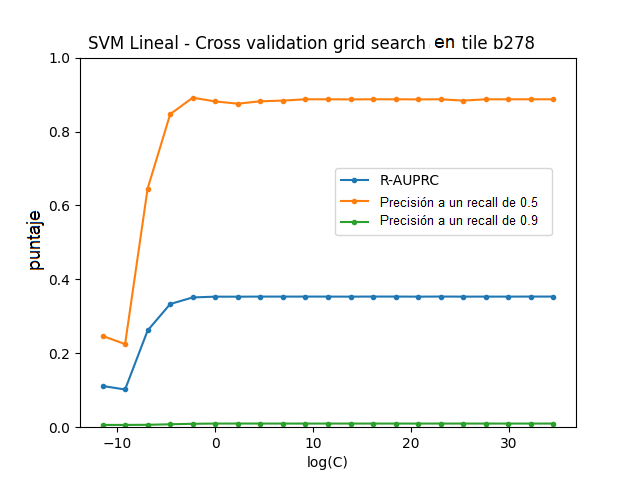
\includegraphics[width=.6\textwidth]{Kap3/Figure_1.png}
  \end{center}
  \caption{Resultados de la optimización de hiperparámetros de SVM-Lineal en el tile b278}
  \label{fig:optimisationsvml}
\end{figure}


\section{Aproximando SVM Kernel}
En la sección \ref{trick} se introdujo el truco del kernel, que consiste en mapear puntos desde un espacio de menor dimensionalidad a un espacio de mayor dimensionalidad. Un punto clave es que, en realidad, únicamente se computan los productos internos en el espacio de mayor dimensionalidad, y nunca es necesario mapear los datos realmente a este espacio. \\

Sin embargo, una de las características de los algoritmos que utilizan este tipo de truco, como SVM kernel, es que su complejidad temporal escala con el número de instancias de entrenamiento ($\mathcal{O}(n^3)$), en tanto que la complejidad espacial será cercana a $\mathcal{O}(n^2)$. Esto vuelve prohibitivo utilizar SVM kernel en los tiles de Carpyncho, que tienen cientos de miles de instancias cada uno. \\

En resumidas cuentas, SVM kernel funciona muy bien en datos que no son linealmente separables, pero no escala bien a datasets con muchas instancias. Por otro lado, como se mencionó en la sección anterior, existen implementaciones de SVM Lineal que escalan de forma lineal a la cantidad de instancias de entrenamiento. \\

Una tendencia reciente es combinar ambos, dejando de lado la idea fundamental del truco del kernel. La idea base es mapear los datos literalmente a un espacio de mayor dimensionalidad y luego aplicar un clasificador lineal, el cuál generará fronteras de decisión no lineales en el espacio original. \\

Dado que algunos kernels, como RBF, mapean los datos a un espacio de infinitas dimensiones; se busca mapear los datos a un espacio con una cantidad finita razonablemente grande de dimensiones. Afortunadamente, se sabe que únicamente un subespacio finito de este espacio con infinitas dimensiones es necesario para resolver el problema de SVM: el espacio inducido por las imágenes de los datos de entrenamiento. \\

Sin embargo, mapear a este espacio inducido sería al menos tan costoso como SVM kernel exacto. Una solución aproximada es utilizar solo un subconjunto de $m<n$ puntos de entrenamiento para generar un mapeo a $\mathbb{R}^m$. Este algoritmo es llamado Método de Nystroem, y permite obtener un mapeo aproximado, pudiéndose controlar la complejidad asociada ajustando el parámetro $m$. \\

Los detalles del procedimiento recien descripto pueden consultarse en las siguientes publicaciones: \cite{nystroem}, \cite{NIPS2012_621bf66d}, \cite{NIPS2007_013a006f}.

\section{Optimización de hiperparámetros para SVM RBF}

En este segundo experimento, se utilizó SVM con un kernel no lineal: Radial Basis Function. La optimización de hiperparámetros se vuelve significativamente más costosa, dado que se deben optimizar los parámetros $C$ y $\gamma$ en simultáneo. Como ya se mencionó, debido al inmenso tamaño de nuestros tiles (aproximadamente 400000 filas cada uno), resultó imposible utilizar implementaciones puras de kernel SVM. \\

Se decidió utilizar un aproximador del kernel RBF, Nystroem con $m=300$, seguido de la eficiente implementación de LinearSVC descripta en la sección anterior. Esto permite aproximar los resultados de kernel SVM, reduciendo dramáticamente la complejidad computacional requerida.\\

Durante el experimento, se realizó 10-fold Grid Search Cross Validation sobre el tile b278. Se exploró un amplio rango logarítmico de valores para los hiperparámetros $\alpha$ y $C$. Los resultados pueden observarse en \ref{fig:optimisationsvmk}. \\

\begin{figure}[h!]
\begin{tabular}{cc}
  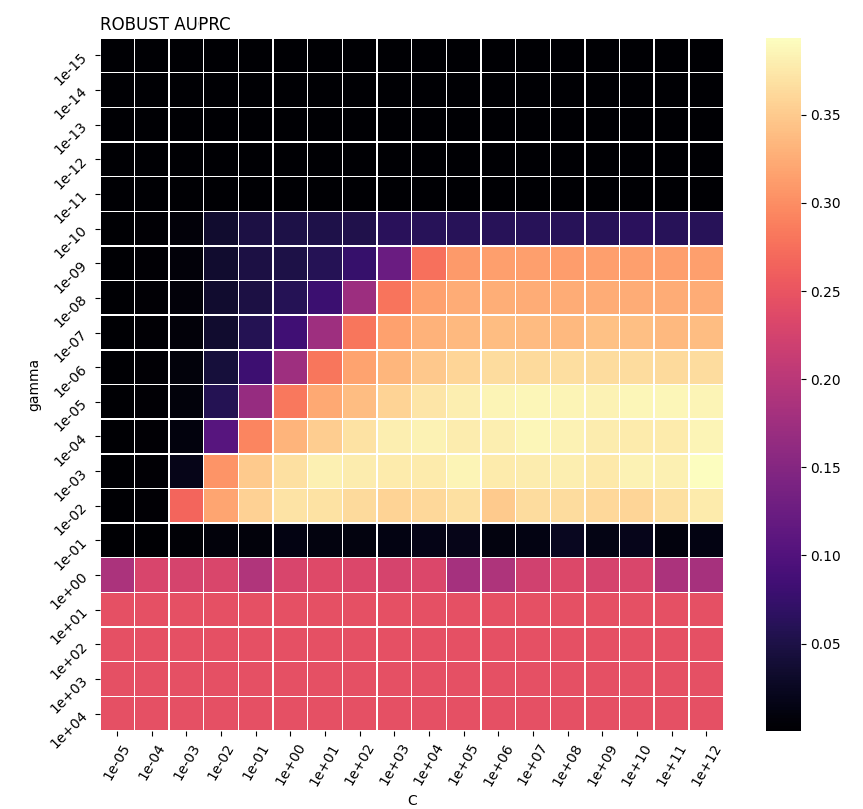
\includegraphics[width=0.49\textwidth]{Kap3/Figure_2.png} &   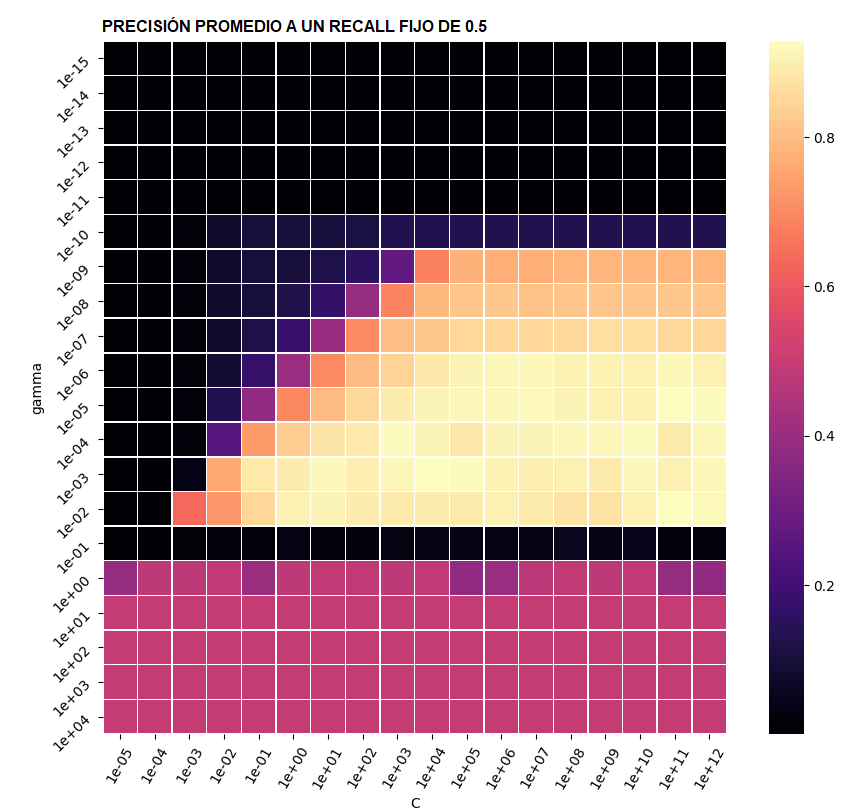
\includegraphics[width=0.49\textwidth]{Kap3/Figure_3.png} \\
(a) Area bajo la curva de Precision-Recall & (b) Precision a un recall fijo de 0.5 
\end{tabular}
\caption{Resultados de la optimización de hiperparámetros para SVM-RBF en el tile b278}
\label{fig:optimisationsvmk}
\end{figure}


Podemos observar que SVM-RBF es muy sensible a la elección de hiperparámetros, a diferencia de RF que no se ve muy afectado por la elección del número de árboles. Los hiperparámetros óptimos fueron $C=10^5$ y $\gamma=10^{-4}$.

\section {Análisis de performance de SVM}

Habiendo estimado los hiperparámetros óptimos de SVM con kernel lineal y RBF, se procedió a entrenar y testear clasificadores usando cada par de tiles en \{ b234, b261 , b278, b360 \}. Las curvas de precision-recall de ambos modelos, así como las de RF, pueden observarse en la figura \ref{fig:testresults}. \\

\begin{figure}[h!]
\begin{center}

\begin{tabular}{ccc}
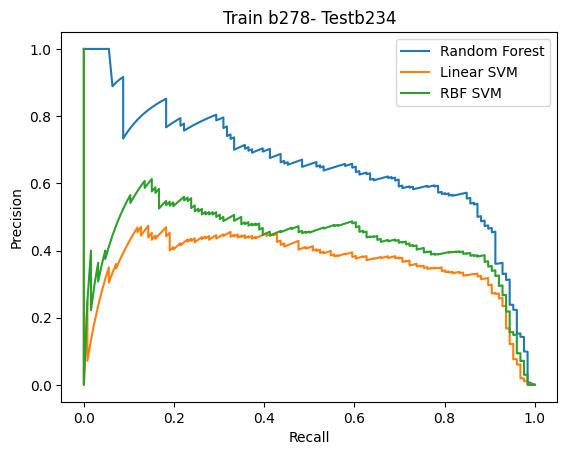
\includegraphics[width=0.32\textwidth]{Kap3/test_results_train=b278Test=b234.png} &
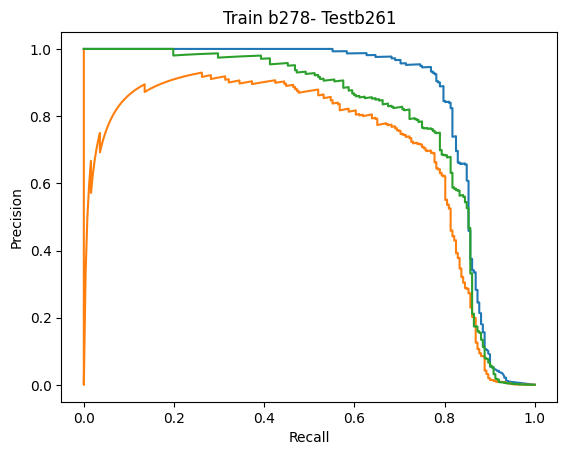
\includegraphics[width=0.32\textwidth]{Kap3/test_results_train=b278Test=b261.png} &
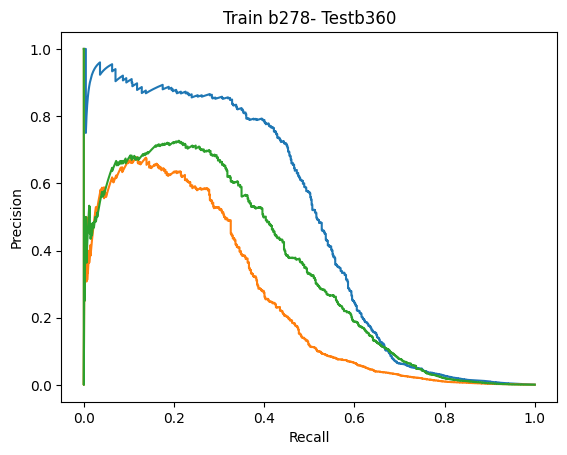
\includegraphics[width=0.32\textwidth]{Kap3/test_results_train=b278Test=b360.png} \\

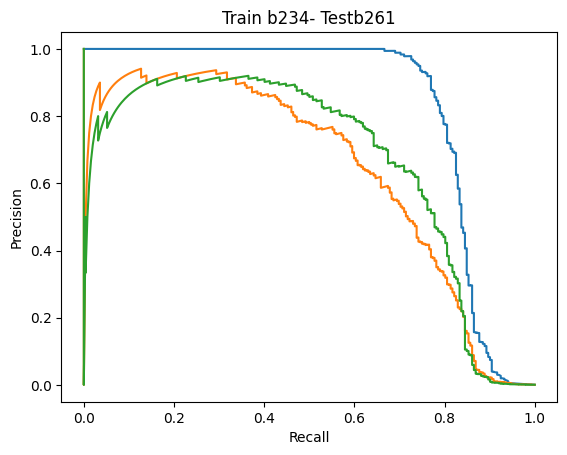
\includegraphics[width=0.32\textwidth]{Kap3/test_results_train=b234Test=b261.png} &
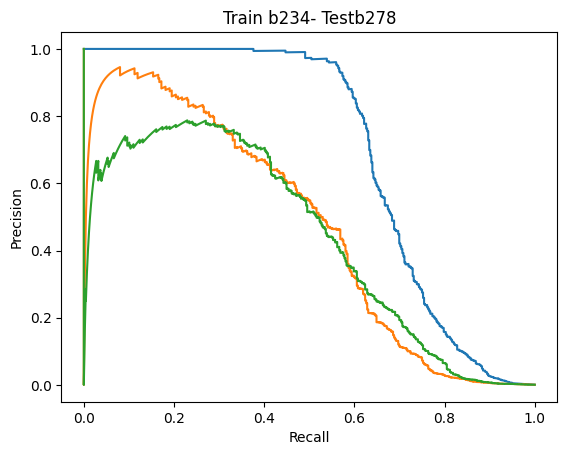
\includegraphics[width=0.32\textwidth]{Kap3/test_results_train=b234Test=b278.png} &
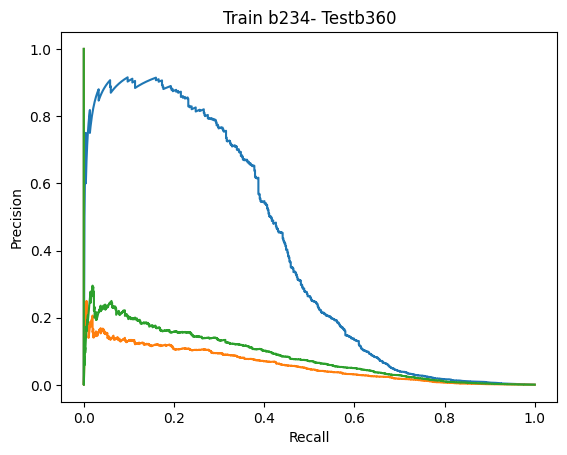
\includegraphics[width=0.32\textwidth]{Kap3/test_results_train=b234Test=b360.png} \\

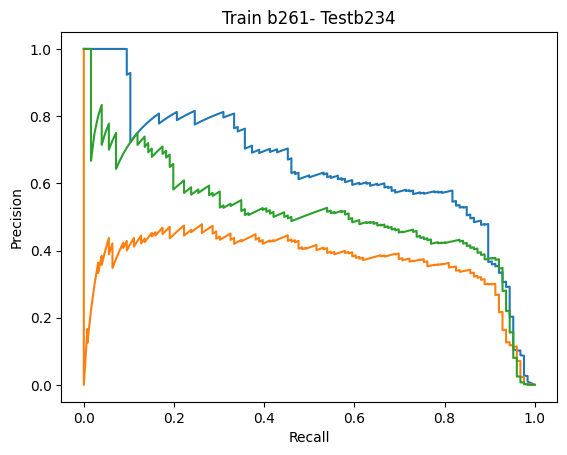
\includegraphics[width=0.32\textwidth]{Kap3/test_results_train=b261Test=b234.png} &
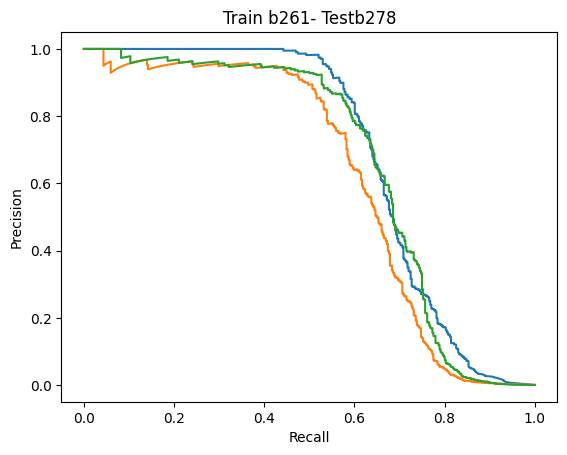
\includegraphics[width=0.32\textwidth]{Kap3/test_results_train=b261Test=b278.png} &
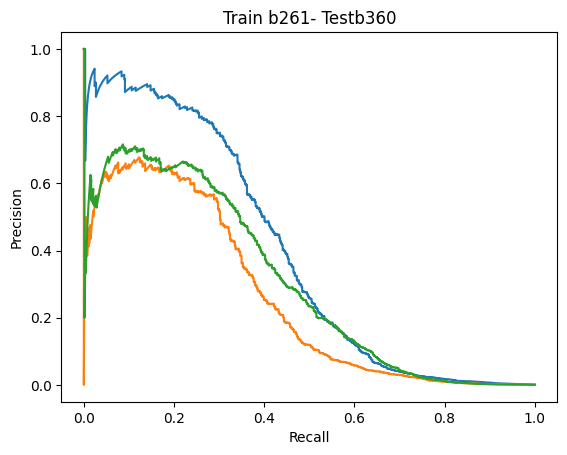
\includegraphics[width=0.32\textwidth]{Kap3/test_results_train=b261Test=b360.png} \\

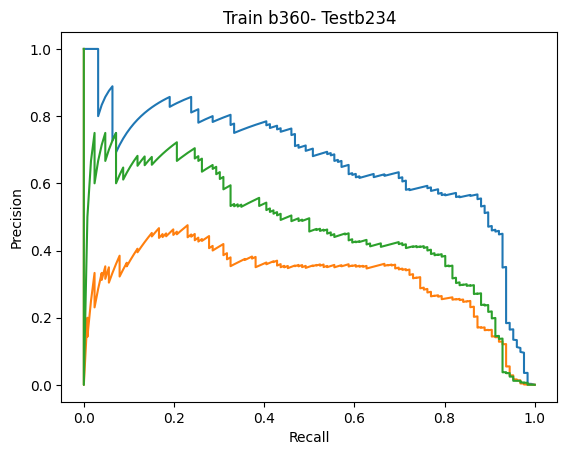
\includegraphics[width=0.32\textwidth]{Kap3/test_results_train=b360Test=b234.png} &
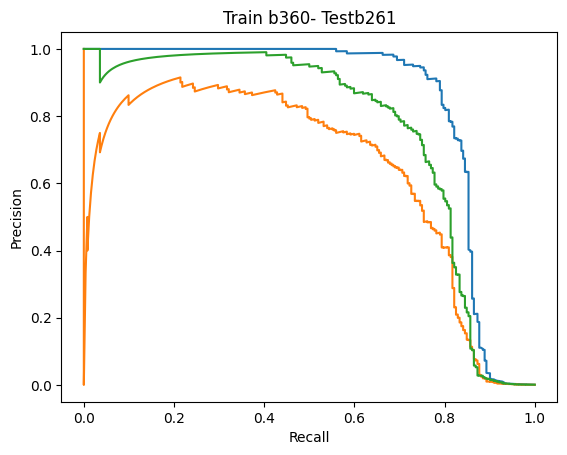
\includegraphics[width=0.32\textwidth]{Kap3/test_results_train=b360Test=b261.png} &
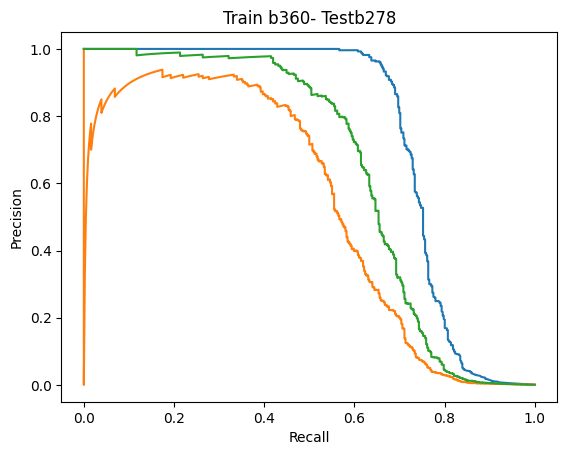
\includegraphics[width=0.32\textwidth]{Kap3/test_results_train=b360Test=b278.png}

\end{tabular}

\end{center}
\caption[short]{Curvas de precision-recall obtenidas utilizando Random Forest, Support Vector Machine con kernel lineal y Support Vector Machine con kernel RBF}
\label{fig:testresults}

\end{figure}

\newpage
Algunas observaciones:

\begin{itemize}

\item En las 12 combinaciones testeadas la performance de random forest es superior a la de SVM-RBF, la cuál es a su vez superior a SVM Lineal. Esto se condice con los resultados reportados en \cite{jbc}. El hecho de haber utilizado las tiles completas para entrenar y testear nos permite apreciar con exactitud cuán mejores son las curvas generadas por Random Forest, lo cual no era evidente en trabajos previos.

\item El hecho de que SVM Lineal tenga la menor performance parece indicar que la superficie de decisión no es lineal.
\item El hecho de que las curvas varíen tanto para cada par de tiles elegido, indica que los clasificadores se ven altamente influenciados por el tile de train y el tile de test elegido. Esto no sucedería si los samples de todos los tiles estuviesen regidos por la misma distribución de probabilidad subyacente. Dado que cada tile tiene cientos de miles de samples, esto indicaría que los datos de cada tile son inherentemente distintos, de otro modo las curvas de cada clasificador deberían ser muy parecidas entre distintos tiles.
\end{itemize}

En los capítulos siguientes se aplicarán distintas técnicas con el objeto de mejorar las curvas obtenidas por SVM. Adicionalmente, se intentará comprender por qué RF parece funcionar mucho mejor que SVM en este tipo de datos.